

%%%%%%%%%%%%%%%%%%%%%%%%%%%%%%%%%%%%%%%%%%%%%%%%%%%%%%%%%%%%%%%%%%%%%%%
\begingroup
\renewcommand{\cleardoublepage}{}
\renewcommand{\clearpage}{}
\vspace{1em}
\chapter{Разработка методики диагностики}
\endgroup
%%%%%%%%%%%%%%%%%%%%%%%%%%%%%%%%%%%%%%%%%%%%%%%%%%%%%%%%%%%%%%%%%%%%%%%
В ~\cite{ontoapproach} описывается подход использующий онтологическое моделирование для диагностики систем хранения данных. Рассмотрим подробнее данный подход. 

В  онтологической  модели  функционирования СХД используется иерархическое представление СХД, в котором каждый из вышележащих компонентов СХД состоит из одного или более нижележащих компонентов (онтологическое отношение consistOf) (рисунок ~\ref{fig:onto}).
\begin{figure}[h]
	\centering
	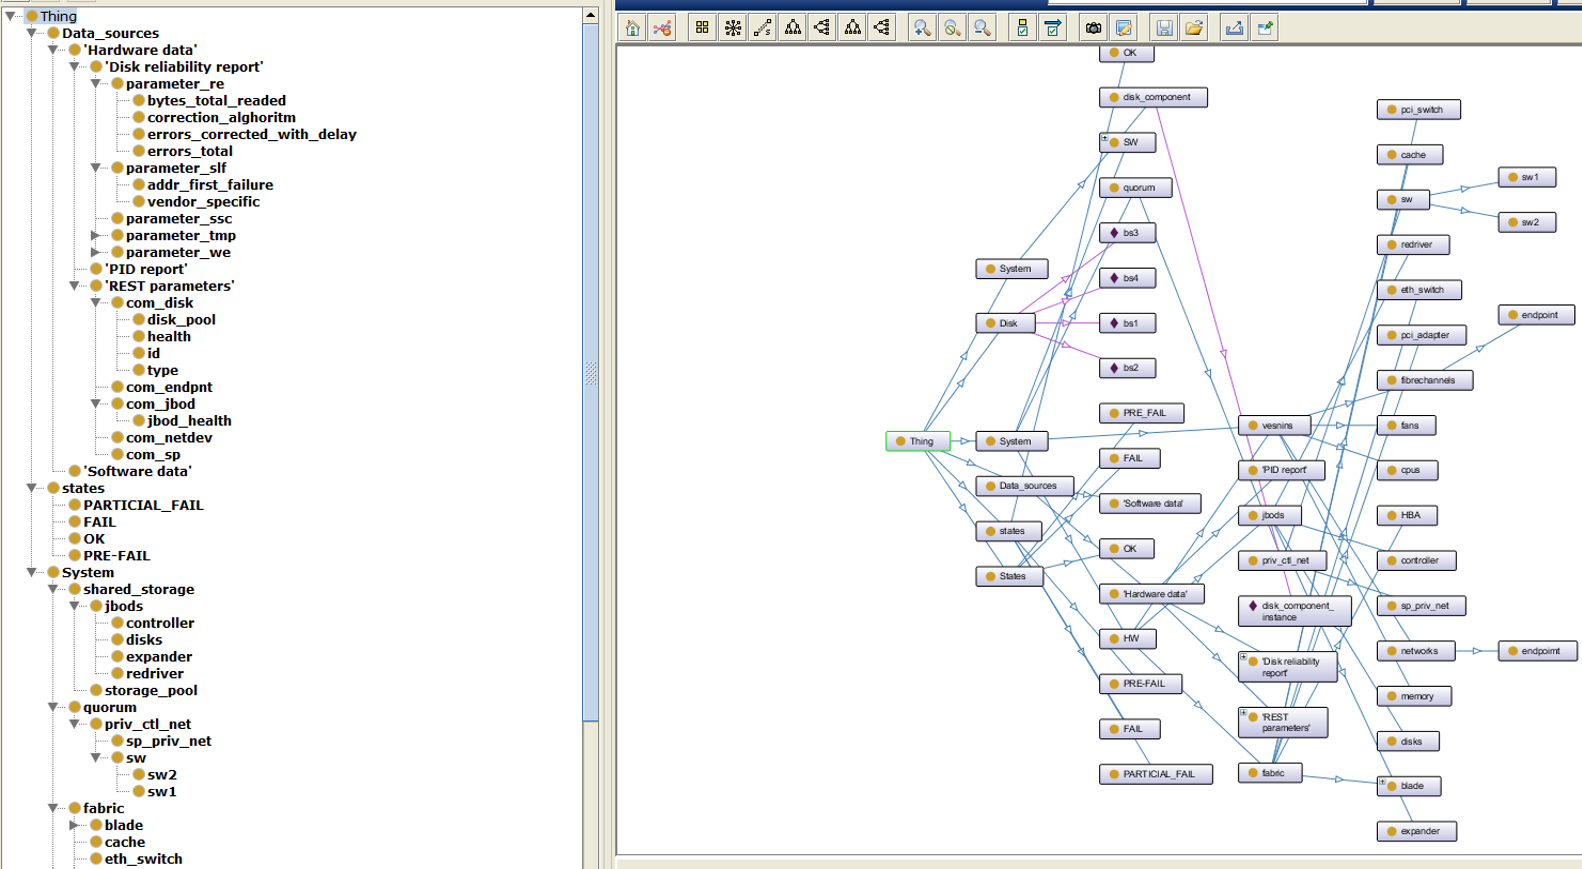
\includegraphics[width=\textwidth]{onto}
	\caption{Пример топологии системы}
	\label{fig:onto}
\end{figure}

Каждый нижележащий компонент влияет на  состояние  вышележащего  компонента,  при  этом  степень  влияния определяется кардинальностью связи consistOf. Например, для поддержания работоспособности внутренней сети (PrivateNetwork) необходимо,  чтобы входящий  в  её  состав  компонент “Виртуальный коммутатор  внутренней  сети”  (VirtualSwitch)  находился  в  работоспособном состоянии,  в  то  время  как  для  нескольких  интерфейсов  подключения контроллера  к  внутренней  сети–PrivateNetworkInterface(количество интерфейсов  равно  числу  контроллеров),  достаточно  лишь  большей  части работоспособных.

На нижнем  уровне  топологии  располагаются  элементарные компоненты  (ElementaryComponent).  Каждый  элементарный  компонент связан  только  с  одним  параметром,  на  основе  которого вычисляется состояние элементарного компонента.Таким  образом,  алгоритм  диагностирования СХД включает  в  себя решение двух подзадач:
\begin{itemize*}
	\item{оценку состояния  элементарного  компонента  на  основе  значения связанного с ним параметра;}
	\item{восстановление состояний вышележащих компонентов (в том числе системы в целом) на основе состояний нижележащих компонентов.}
\end{itemize*}
Для определения состояния компонента СХД необходимо определить все  нижележащие  компоненты,  входящие  в  состав  анализируемого компонента и вычислить их состояния.Состояние СХД в целом аналогично определяется как состояние всех компонентов СХД верхнего уровня.

Вычисление  состояния  компонентов  выполняется  при  помощи функции вычисления работоспособности компонента на основании экспертных знаний о компоненте.

На основании данного подхода предлагается методика диагностики состояний дисков????
Общая структура методики???? представлена на рисунке ~\ref{fig:DiagModule}.
\begin{figure}[h]
	\centering
	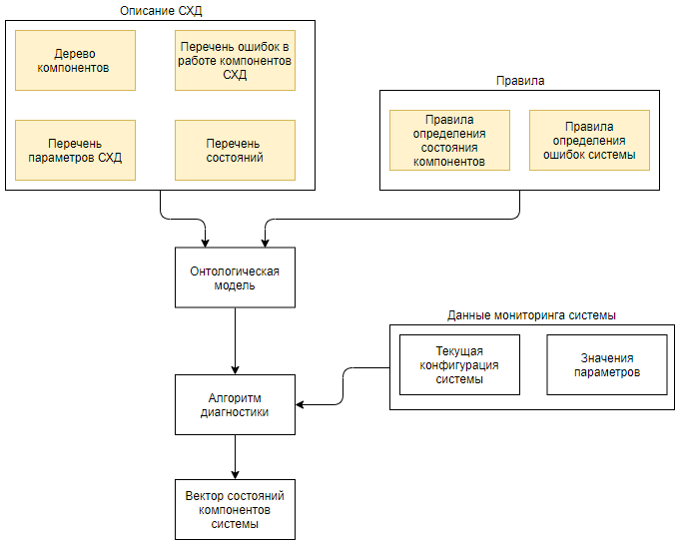
\includegraphics[width=\textwidth]{DiagModule}
	\caption{Общая схема получения параметров для модели}
	\label{fig:DiagModule}
\end{figure}

Методика построения owl модели на примере SMART параметров дисков и климатических параметров представлена на рисунке ~\ref{fig:DataSources}.

\begin{figure}[h]
	\centering
	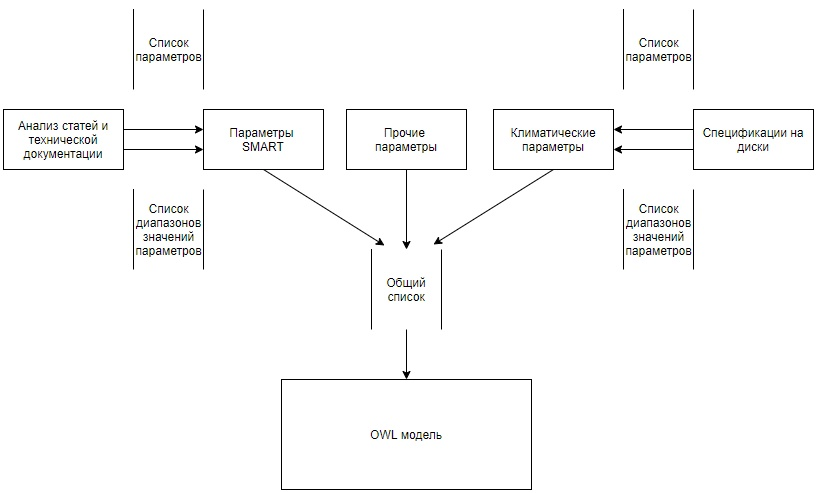
\includegraphics[width=\textwidth]{DataSources}
	\caption{Общая схема получения параметров для модели}
	\label{fig:DataSources}
\end{figure}

Согласно сформированным задачам рассмотрим каждую из них: 
\begin{itemize*}
	\item{Анализ объекта диагностики}
	\item{Определение параметрического пространства для объекта диагностики}
	\item{Описание возможных состояний объекта диагностики}
	\item{Определение значений параметров соответствующих различным состояниям объекта диагностики}
	\item{Формирование диагностической модели}
\end{itemize*}

Анализ объекта диагностики был выполнен в первой главе данной работы. 

Ниже приведено исследование статей и публикаций, что в результате формирует список параметров со знчениями для наполнения онтологической модели.

\section{Определение параметрического пространства для объекта диагностики}

%%%%%%%%%%%%%%%%%%%%%%%%%%%%%%%%%%%%%%%%%%%%%%%%%%%%%%%%%%%%%%%%%%%%%%%%%%%%%
\subsection{HDD диски}
%%%%%%%%%%%%%%%%%%%%%%%%%%%%%%%%%%%%%%%%%%%%%%%%%%%%%%%%%%%%%%%%%%%%%%%%%%%%%
Традиционно состояние HDD дисков оценивается на основании статистического показателя MTBF - среднего времени наработки на отказ, который указывается производителем в специикации. Однако, в последнее время, производители перешли к метрике AFR - пересчитанная на год интенсивность отказов. Данную метрику можно использовать при оценке состояния жестких дисков совместно с показателем суммарной наработки.  

Распростаненными оценками MTBF являются 300000-1200000 часов, что соответсвует 30-120 годам беспрерывной работы устройств. Расчет данной метрики производится на основании испытания большого количества дисков, постоянно работающих на испытательной площадке производителя, с последущей экстраполяцией результатов. 
Распространенные оценки AFR - 0.5-1%. 
Также, надежность жесткого диска тесно связана с климатическими параметрами окружающей его среды. 
Рассмотрим для примера один из используемых в исследуемой СХД HDD дисков - HGST Ultrastar 7K6000~\cite{HGST}. На рисунке ~\ref{fig:temp} приведен график рабочего диапазона температур и высоты над уровнем моря для рассматриваемого диска. Аналогичные показатели с небольшими отклонениями(не более 5 градусов цельсия и 500м высоты) приводят и другие производители, что связано со схожими технологиями производства и применяемыми компонентами. 

\begin{figure}[!h]
	\centering
	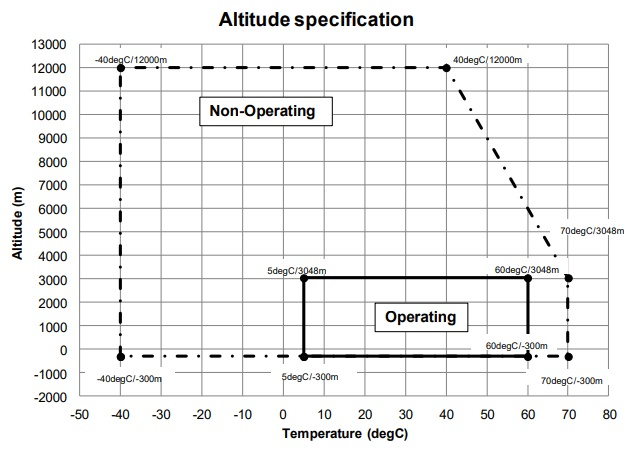
\includegraphics[width=\textwidth]{temp}
	\caption{График предельных значений высоты над уровнем моря от температуры для диска HGST Ultrastar}
	\label{fig:temp}
\end{figure}

Кроме того, важным показателем окружающей среды, влияющим на срок службы жосткого диска является влажность. График рабочих диапазонов влажности от температуры (см. рисунок ~\ref{fig:temp}) демонстрирует резкое снижение рабочего порога влажности при увеличении температуры начиная с 30 градусов цельсия. 

Основываясть на знаниях о принципе действия жестких дисков можно предположить, что такой параметр как уровень вибрации на корпусе диска может также повлиять на срок его службы. Это может быть связано с ускорением износа механической части (подшипников в двигателе, опорных подшипков).

\begin{figure}[!h]
	\centering
	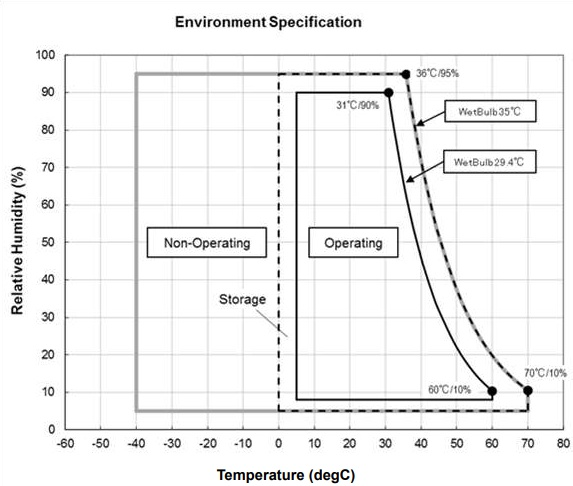
\includegraphics[width=\textwidth]{hum}
	\caption{График предельных значений влажности от температуры для диска HGST Ultrastar}
	\label{fig:hum}
\end{figure}

Таким образом, вышеупомянутые параметры давления(напрямую связано с высотой над уровнем моря), влажности, температуры и вибрации являются важной частью мониторинга состояния HDD дисков. 

Одним из основополагающих при дисгностике состояния диска является чтение параметров SMART(Self-Monitoring, Analysis and Reporting Technoogy). В настоящее время 
технология  SMART  встроена  в  каждый  диск  и  сообщает  о  различных 
атрибутах,  связанных  с  надежностью  жесткого  диска. Изготовитель  может 
использовать данные, полученные SMART, чтобы локализовать недостатки и 
предотвратить их повторение в будущих моделях дисков. Каждый SMART 
атрибут   представлен   не обработанным и нормированным значением, однако они могут иметь различную интерпретацию в зависимости 
от конфигурации жесткого диска, поэтому отсутствует надежный механизм 
для  определения  того,  какой  из  SMART  атрибутов  является  лучшим 
индикатором сбоя диска. 

В ~\cite{diskred} для анализа дисковых накопителей использованы открытые данные из Backblaze,  полученные  по  технологии SMART.  В Backblaze собираются  данные SMART,  получаемые  от диска  раз  в день.  Эти данные не хранят информацию о точном месте появления ошибки. Поэтому считается, что с большой вероятностью ошибки случаются непосредственно в или рядом с теми адресами, в которых ранее наблюдались симптомы или ошибки.

В таблице~\ref{tab:smart} представлены результаты тестовых испытаний СХД по технологии SMART для параметров, проявивших корреляцию с выходом из сроя диска.
\begin{table}
	\captionsetup{skip=5pt}
	\caption{Результаты тестовых испытаний дисков с технологией SMART}
	\centering
	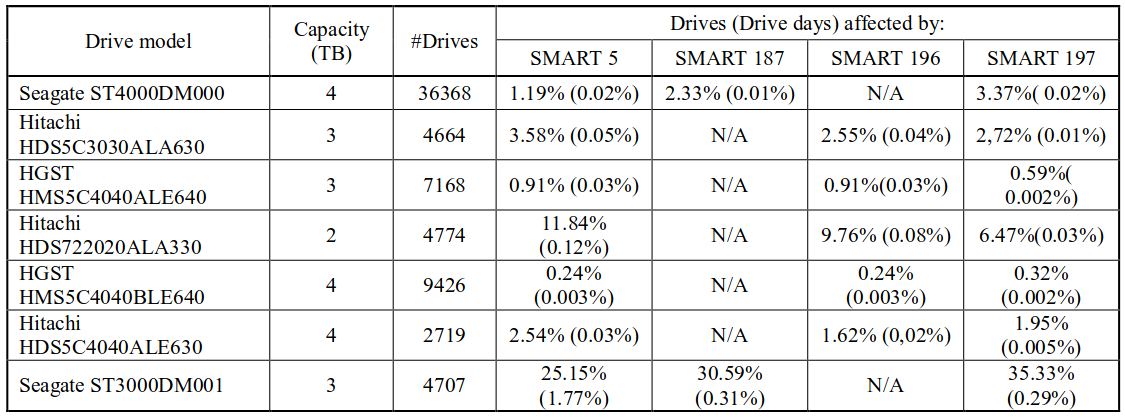
\includegraphics[width=\textwidth]{table}
	\label{tab:smart}
\end{table}
\begin{itemize*}
	\item{SMART 5:  Число  переназначенных  секторов  (reallocated sectors).  Когда 
невозможно чтение или запись сектора, диск помечает сектор как испорченный (bad) и перемещает его (remap, reallocate) на запасной сектор диска.}
	\item{SMART 187:  Число  ошибок  чтения,  которые  не  смогли  быть  исправлены 
аппаратным помехоустойчивым кодом.}
	\item{SMART 196:  Общее  число  попыток  передачи  данных  из  переназначенных 
секторов в запасные. Считаются как неуспешные, так и успешные попытки.}
	\item{SMART 197:  Число «нестабильных» секторов.  Некоторые  диски  после 
неудачного  чтения  помечают  сектор  как «нестабильный»,но  переназначают  его 
только  через  некоторое  время,  убедившись  в  том,  что  данные  не  могут  быть 
восстановлены при последующем чтении или перезаписи новыми данными.} 
\end{itemize*}

Таким образом, определен перечень наиболее значимых SMART параметров, которые в совокупности с климатическими параметрами будут использоваться для  диагностики состояний HDD дисков. 
%%%%%%%%%%%%%%%%%%%%%%%%%%%%%%%%%%%%%%%%%%%%%%%%%%%%%%%%%%%%%%%%%%%%%%%%%%%%%
\subsection{SSD дииски}
%%%%%%%%%%%%%%%%%%%%%%%%%%%%%%%%%%%%%%%%%%%%%%%%%%%%%%%%%%%%%%%%%%%%%%%%%%%%%

В статье ~\cite{reliabil} авторами рассматривается вопрос надёжности SSD дисков, на основании NAND ячейки, произведённых по различным технологиям.

Для ясности дадим определение двум рассматриваемым метрикам:
\begin{itemize*}
	\item{UBER (uncorrectable bit error rate= uncorrectable bit readed/total bit readed}
	\item{RBER (raw bit error rate)= N corrupted bits / N bits readed}
\end{itemize*}
Зачастую, в различных исследованиях и докладах ~\cite{art} о надежности SSD дисков для оценки состояния носителя используется именно эта метрика. 
Однако, метрика UBER не является хорошим инструментом для оценки состояния диска. Алгоритмическое исправление ошибок чаще всего реализовано циклически, поэтому прежде чем ячейка будет исправлена, каждое чтение из неё будет увеличивать значение в числителе. Таким образом числитель и знаменатель коррелируют, вводя в заблуждение исследователей. 

По вышеописанной причине, авторы предлагают использовать метрику RBER. 


Среди результатов исследования также значится:
\begin{itemize*}
	\item{97\% дисков имеет битые ячейки памяти ещё со стадии производства. Их количество зависит от производителя и модели} 
    \item{От 2 до 7\% исследуемых дисков имели бите чипы}
    \item{Чаще всего, в случае одновременного выхода из строя парного количества ячеек, виноват чип} 
    \item{Определены параметры для диагностики состояния диска:}
	\begin{enumerate}
		\item{Ошибки данных (обнаруженные CRC, и пр.)}
		\item{Ошибки чтения/записи}
		\item{Ошибки отключения SATA}
		\item{Количество переназначенных секторов}
	\end{enumerate}
\end{itemize*}

Результаты исследования, с указанием процента устройств, вышедших их строя с обозначенными параметрами, отклоняющимися от нормальных значений, показаны на рисунке ~\ref{fig:failed}. Как видно из рисунка, наиболее точным признаком среди исследованных является количество переназначенных секторов, что напрямую связано с количеством неисправленных бит.
Значение метрики RBER= 1e-08 – 1e-03(чаще всего 1е-06) наблюдалось у устройств, непосредственно перед выходом из строя, а, следовательно, может быть использовано как опорное в целях диагностики состояния диска.

\begin{figure}[h]
	\centering
	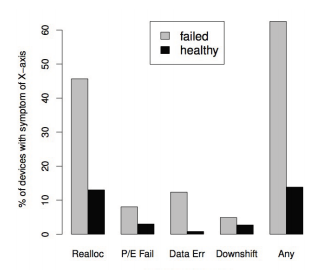
\includegraphics[width=3.0in]{failed}
	\caption{Процент вышедших из строя устройств 
с указанными симптомами}
	\label{fig:failed}
\end{figure}

В статье ~\cite{faildatacenter} исследователи из компании Microsoft также систематизировали возникающие выходы из строя дисков и связали их с наблюдаемыми параметрами. 
В результате, выделяется четыре наиболее важных симптома для определения состояния SSD:
\begin{itemize*}
	\item{Ошибки данных}
    \item{Переназначение секторов}
    \item{Ошибки чтения/записи}
    \item{Ошибки отключения SATA}
\end{itemize*}
Представленный выше набор симптомов сходится с аналогичным набором выше от других исследователей. 
Кроме того, определяется степень важности характеристик для идентификации состояния диска по категориям (см. рисунок ~\ref{fig:params}). 
\begin{figure}[!h]
	\centering
	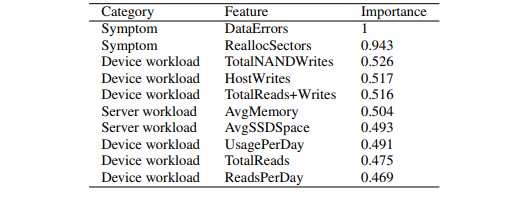
\includegraphics[width=\textwidth]{params}
	\caption{Важность исследуемых характеристик в 
		диагностике состояния устройства}
	\label{fig:params}
\end{figure}

Также в ходе исследования были получены следующие результаты:
\begin{itemize*}
	\item{80\% здоровых устройств имеют <2 переназначенных секторов}
    \item{Если сообщения о сбое основаны на внутренних ошибках/проблемах, то чаще всего устройство выйдет из строя в течении месяца. Если сообщения о сбое основаны на большой нагрузке на устройство – чаще всего устройство функционирует дольше месяца}
    \item{Около 62\% вышедших из строя устройств имеют как минимум один из 4 проявившийся симптом. При этом оставшиеся 38\% не демонстрируют наличие проявления обозначенных симптомов} 
    \item{Определён ряд паттернов на основе различных метрик для оценки состояния диска. Пример представлен на рисунке ~\ref{fig:patterns}. Параметр MediaWearout приведен к шкале 1-100(100- новый диск, 1- полностью изношен)}
\end{itemize*}

\begin{figure}[h]
	\centering
	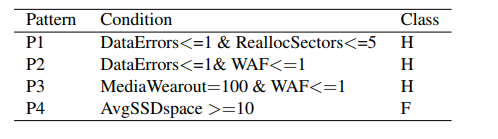
\includegraphics[width=\textwidth]{patterns}
	\caption{Пример паттернов определения состояния диска}
	\label{fig:patterns}
\end{figure}
 

Где WAF - write amplification –отношение количества записанных данных на диск к количеству данных отправленному на запись на хосте.
Столбец Class отображает класс, к которому стоит отнести устройство с удовлетворяющими правилу параметрами (H – Healthy-здоровый, F – Failure- неисправный).

Кроме того, в  ~\cite{errorpredr} описано исследование 7 моделей дисков с целью определения параметров, позволяющих определять состояние диска. Кроме упоминаемых ранее, в нем фигурируют такие параметры как ошибки фабрики, недельные статистики циклов записи и количества плохих секторов.
\begin{table}
	\captionsetup{skip=5pt}
	\caption{Агрегированный набор параметров 
		для определения состояния SSD диска}
	\centering
	\begin{tabular}{ | l | l | }
		\hline
		ID & Parameter Name \\ \hline
		1 & correctable error  \\
		2 & erase count \\
		3 & erase error \\
		4 & factory bad blocks\\
		5 & final read error\\
		6 & final write error\\
		7 & meta error\\
		8 & PCI Bus Power Consumotion\\
		9 & read count\\
		10 & read error\\
		11 & response error\\
		12 & status dead\\
		13 & status read only\\
		14 & temperature\\
		15 & timeout error\\
		16 & total NAND writes\\
		17 & uncorrectable error\\
		18 & write count\\
		19 & write error\\
		20 & comulative bad block count fixed\\
		21 & weekly bad block count\\
		22 & comulative program/erase cycle fixed\\
		23 & weekly program/erase cycle\\
		\hline
	\end{tabular}
	\label{table:tab1}
\end{table}

В таблице  ~\ref{table:tab1} представлен агрегированный список параметров составленный на основании рассмотренных статей. Данные параметры представляют наибольший интерес при диагностике SSD дисков. 

\section{Описание возможных состояний объекта диагностики}
Рассмотрим возможные состояния компонентов системы в соответствии с ГОСТ 27.002–2015:
\begin{itemize*}
	\item{работоспособное состояние;}
	\item{предотказное состояние (сбой);}
	\item{неработоспособное состояние (частичный отказ);}
	\item{предельное состояние (полный отказ).}
\end{itemize*}
Под работоспособным состоянием понимается такое состояние системы,в котором она способна выполнять все требуемые функции. 
Предотказное состояние - это состояние системы, характеризуемое повышенным риском ее отказа. 
Неработоспособное состояние - это состояние системы при котором она не способна выполнять хотя бы одну требуемую функцию.
Под предельным состоянием понимается такое состояние системы, при котором ее дальнейшая эксплуатация недопустима или нецелесообразна. 

\section{Определение значений параметров соответствующих различным состояниям объекта диагностики}
В соответствии с предыдущим пунктом данной работы определим каждому возможному состоянию системы набор параметров и значений его характеризующих на примере климатических параметров. Так, на основании спецификаций (см. рисунок~\ref{fig:temp}-~\ref{fig:hum}) определим:
Работоспособное состояние:
\begin{itemize*}
	\item{от +10\degreeС до +55\degreeС,}
	\item{от -250м до 3000м над уровенем моря},
	\item{от 8 до 90\% при температуре от 5\degreeС до 30\degreeС, по соответствующей кривой при температурах от 30\degreeС до 60\degreeС максимальная влажность снижается до 10\%}
\end{itemize*} 
Предотказное состояние: 
\begin{itemize*}
\item{от +5 до +10 и от +55\degreeС до +60\degreeС,}
\item{от -300 до -350 и от 3000 до 3048м над уровенем моря,}
\item{от 5 до 10 и от 90 до 95 \% при температурах от 0\degreeС до 30\degreeС градусов}
\end{itemize*} 
Частичный отказ: 
\begin{itemize*}
\item{от -40\degreeС до +5\degreeС и от +60\degreeС до +70\degreeС,}
\item{от 3048м до 12000м над уровнеем моря, }
\item{ от 5 до 95\% при температуре от 0\degreeС до -40\degreeС}
\end{itemize*} 
Полный отказ: 
\begin{itemize*}
\item{менее -40\degreeС и более 70\degreeС}
\item{более 12000м над уровнем моря или менее -300м над уровнем моря,}
\item{при влажности не подпадающей под предыдущие режимы}
\end{itemize*} 

Для вибрации производители не указывают какие-либо допустимые уровни, поэтому для данного параметра необходимо проводить исследования.

\section{Формирование диагностической модели}
Для обеспечения полноты собираемых параметров был разработан АПК сбора климатических параметров, который обеспечивает рассматриваемую модель значениями климатических параметров(температура, давление,влажность, вибрация). Исходя из спецификаций используемых в СХД дисков были определены граничные значения гарантированной работы устройств и занесены в онтологическую модель (см. рисунок ~\ref{fig:DataParam}). 

\begin{figure}[h]
	\centering
	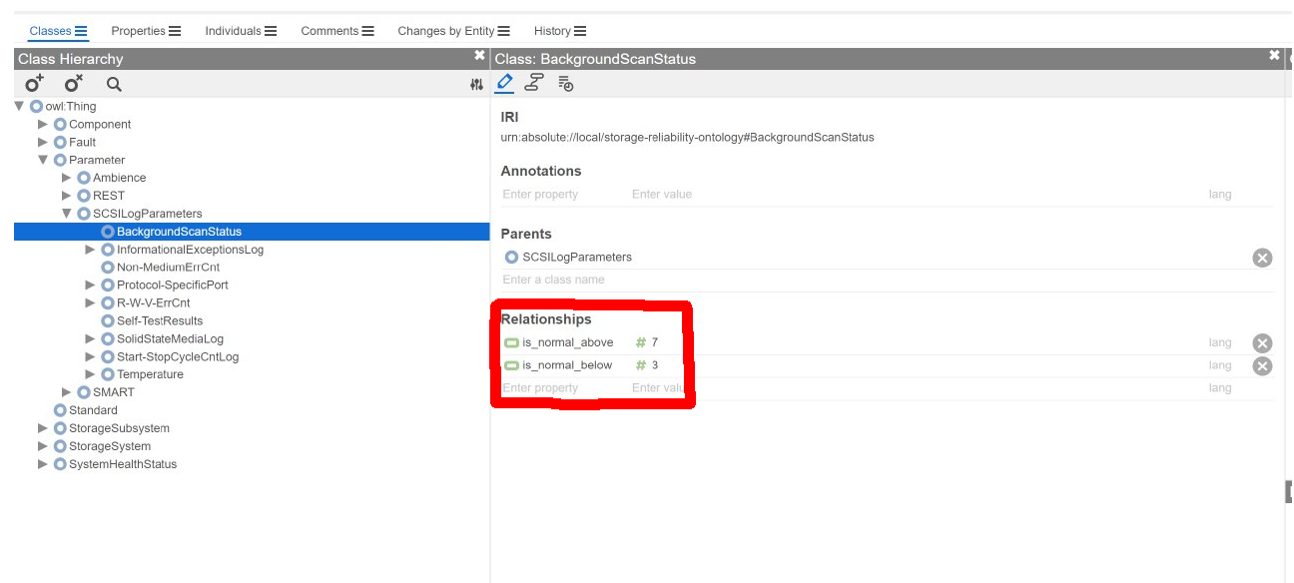
\includegraphics[width=\textwidth]{DataParam}
	\caption{Установка граничных значений параметров для модели}
	\label{fig:DataParam}
\end{figure}